\section{Background}
\label{background}
Finishing my thesis project required knowledge from many different areas and courses.
I needed the contents of Information Security I and II, as well as those of Compiler Construction and Advanced C++ Programming.
This section will give a brief introduction to the relevant topics from those courses.

\subsection{Power Analysis Attacks}
In most cases the power consumption during execution is data-dependent.
Setting a bit to 1 requires more power than setting it to 0, and power consumption is thus directly linked to the \hammingw{} of processed data.
While this connection is very hard to observe in real time, it is easy to detect using statistical analysis of the power consumptions of multiple executions.
For easier analysis, the power consumption is quantized and stored in numerical format as a so-called power trace.

Embedded devices are often exposed to this kind of attack, as an attacker has physical access to the device.
Their power consumption is also fairly low in noise, as they lack any kind of parallelism.
Additionally, many use-cases for embedded devices include some cryptographic operation on sent input without much validation, giving the attacker an easy and valuable target for her attack.
\\
\\
An example attack would go like this:
An attacker solders a resistor between the target processor and the ground of its power supply.
She then measures the voltage difference between both ends with an oscilloscope (this voltage is directly proportional to the current flowing through the resistor).
This gives her easy access to the power traces at a high resolution and for every clock cycle.

After the setup, she submits a large number of different plaintexts to the target (\textasciitilde 1000 is a good starting point), collecting the power traces.
She then starts attacking the secret key byte by byte (attacking individual bytes drastically reduces the search space, keeping this attack feasible).
Because she knows the plaintexts, she can calculate the expected power consumption up until a certain point of the cryptographic operation.
She can then calculate the correlation between expected and actual power consumptions, giving her the probabilities for the key byte guesses.
If everything goes correctly, the correct key byte will have the highest probability.
By repeating this process for every byte, the attacker will eventually recover the entire secret key.

\subsection{Power Analysis Defenses}
There is no absolute defense against power analysis attacks.
All defensive measures can do is increase the amount of effort (required number of traces, computation time for analysis, etc.) an attacker requires for a successful attack.

Masking for example is an algorithm specific defensive measure that adds a third factor to the power consumption.
The attacker then has to calculate her correlation for each possible combination of key byte and mask value.
This increases the number of traces she needs to capture (to still provide the same confidence in her analysis) and the computation time of her analysis.

Other defensive measures focus on creating a worse signal to noise ratio for the entire power consumption.
One technique that has gained a lot of traction is \dual{}\cite{sokolov2005design}.
It works by calculating the inverse of every intermediate result along with the actual result.
This, in theory, keeps the power consumption constant and thus independent of the data.

Unfortunately, \dual{} suffers from multiple engineering problems.
The power required to set the value of a bit to 1 is dependent on properties of the underlying transistors, which are subject to variances in manufacturing.\cite{razafindraibe2006formal}
Minimal differences in clock timings between both paths can also reduce the security of \dual{}\cite{baddam2008path}.
Storing the inverse also requires significantly larger circuitry, doubling the circuit size or more\cite{baddam2008path}.

Even with these caveats, \dual{} has the major advantage that once it is applied, \emph{any} code can be run without modifications while still benefiting from the increased robustness.

\subsection{\llvm{}}
\label{llvm}
The \llvm{} compiler infrastructure project\cite{lattner2010llvm} contains a number of subprojects, but for my thesis the \lc{} libraries are the only part that is relevant.
They contain a source and target independent compiler, which can be extended using multiple front- and backends.
This makes \llvm{} the most versatile compiler available.
\Cref{fig:llvm} shows a sketch of the general architecture of \llvm{}.

\begin{figure}[h]
  \centering
  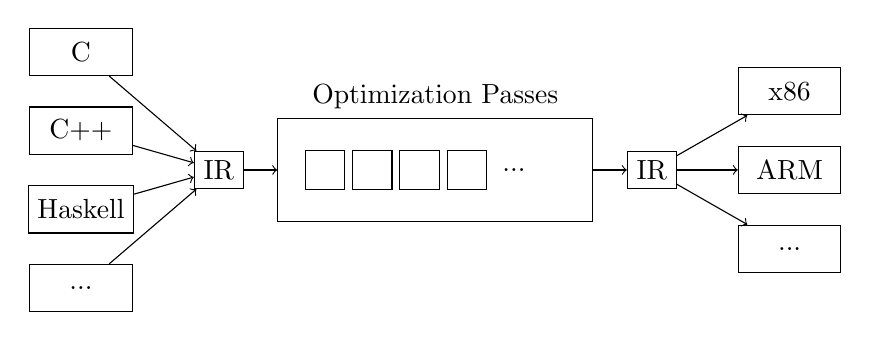
\begin{tikzpicture}
    \node[draw, minimum width=1.3cm, minimum height=0.6cm] at (-2.5,1.5) (C) {C};
    \node[draw, minimum width=1.3cm, minimum height=0.6cm] at (-2.5,0.5) (C++) {C++};
    \node[draw, minimum width=1.3cm, minimum height=0.6cm] at (-2.5, -0.5) (Haskell) {Haskell};
    \node[draw, minimum width=1.3cm, minimum height=0.6cm] at (-2.5, -1.5) (otherl) {...};
    \node[draw] at (-0.75, 0) (irl) {IR};
    
    \node[draw, label=Optimization Passes, minimum width=4cm, minimum height=1.3cm] at (2,0) (optimization) {};
    \node[draw, minimum size=0.5cm] at (0.6,0) {};
    \node[draw, minimum size=0.5cm] at (1.2,0) {};
    \node[draw, minimum size=0.5cm] at (1.8,0) {};
    \node[draw, minimum size=0.5cm] at (2.4,0) {};
    \node at (3.0, 0) {...};

    \node[draw] at (4.75, 0) (irr) {IR};
    \node[draw, minimum width=1.3cm, minimum height=0.6cm] at (6.5,1) (x86) {x86};
    \node[draw, minimum width=1.3cm, minimum height=0.6cm] at (6.5,0) (arm) {ARM};
    \node[draw, minimum width=1.3cm, minimum height=0.6cm] at (6.5,-1) (otherr) {...};

    \draw[->] (C) -- (irl);
    \draw[->] (C++) -- (irl);
    \draw[->] (Haskell) -- (irl);
    \draw[->] (otherl) -- (irl);

    \draw[->] (irl) -- (optimization);
    \draw[->] (optimization) -- (irr);

    \draw[->] (irr) -- (x86);
    \draw[->] (irr) -- (arm);
    \draw[->] (irr) -- (otherr);
  \end{tikzpicture}
  \caption{The general architecture of the \llvm{} compiler}
  \label{fig:llvm}
\end{figure}

At the heart of \lc{} is a number of optimization passes.
These passes take \ir{} as input and provide \ir{} as output.
This allows easy addition and reordering of compiler passes, making it perfect for my thesis.

\llvm{} also has Clang as a frontend, making it an industry-grade C and C++ compiler, which keeps my project from being unusable due to some obscure toolchain.

%% \subsection{Static Single Assignment Form}
%% \label{ssa}
%% In order to understand \ir{} we first need to understand the basics of static single assignment form (SSA).
%% The basic premise of SSA is simple: every value assignment is stored in a new variable.
%% Analysis of variable usage, register requirements (liveness), dead code, etc. is thus greatly simplified.

%% Some notations for SSA annotate the variable names with indices to make them unique.
%% \ir{} completely forgoes the names of variables, instead using just numbers, preceded by a \%.

%% \subsection{\llvm{} Intermediate Representation}
%% \label{ir}
%% \ir{} is best described as typed assembly written in SSA.
%% The instructions provided by \ir{} are very similar to RISC assembly.
%% \ir{} uses SSA variables, which have types associated with them, based on their assignment.
%% This allows typechecking during every step of the compiler, especially between optimization passes.

%% \ir{} also explicitly defines functions with a prototype, complete with typed arguments and return type.

\subsection{\llvm{} C++ API}
\label{api}
\llvm{} provides a C++ API for extending the compiler.
This API exposes all functions that \llvm{} itself uses, giving the programmer full access to all capabilities.
For my thesis I mainly used the code inspection and generation utilities, going through the generated \ir{} code and balancing it, in an optimization pass.

The pass can then be compiled into a library (see \Cref{buildpass}), which is loaded as an \llvm{} plugin during the compilation process.

\subsection{\qemu{}}
\label{qemu}
\qemu{} is a generic and open source machine emulator and virtualizer.\cite{bellard2005qemu}
While it can be used as a full fledged virtualization environment and sandbox, it can also emulate different processor architectures for programs without first emulating an OS.
This process is called bare-metal emulation, and is used for my thesis.

\qemu{} is also open source, allowing for ``easy'' modification and addition of my evaluation code.
Easy is a relative term here, as its size, the complexity of its build process, and its relative lack of documentation make this still a hard problem to tackle.

\subsubsection{Memory Layout of \qemu{} Kernels}
\label{memory}
Even with bare-metal emulation, \qemu{} still takes its input as a kernel.
Due to this, it starts execution at address \hex{1000}, as everything before that address is usually reserved for interrupt handling.
This requires some additional setup in my build process (see \Cref{buildtest}).

\subsection{AES and RC4}
AES\cite{daemen2013design} and RC4\cite{rc4} are the two evaluation programs for my compiler pass.
I chose RC4 because it is very simple and used to be the industry standard, and AES because it is the current industry standard for symmetric encryption.
Both fit the main use cases of embedded devices, and are thus reasonable choices for evaluating the robustness of my thesis project.
